\section{System Model and Architecture}

Power-saving routing in WSNs using a deep reinforcement learning (PSR-DRL) solution aims to solve the main problems of WSNs: making them more energy-efficient and ensuring data is sent reliably. The PSR-DRL solution integrates DRL with established sensor networking techniques to establish a flexible and intelligent framework that enhances the network's lifespan and ensures optimal performance in diverse deployment scenarios.

\subsection{System Architecture Overview}

The PSR-DRL system employs a modular architecture consisting of five specialized modules that work collaboratively to optimize network performance while maximizing network lifetime. Figure~\ref{fig:psr_drl_architecture} illustrates the comprehensive system architecture, showing the interactions between modules and the central role of the DRL module in decision-making.

\begin{figure}[htbp]
    \centering
    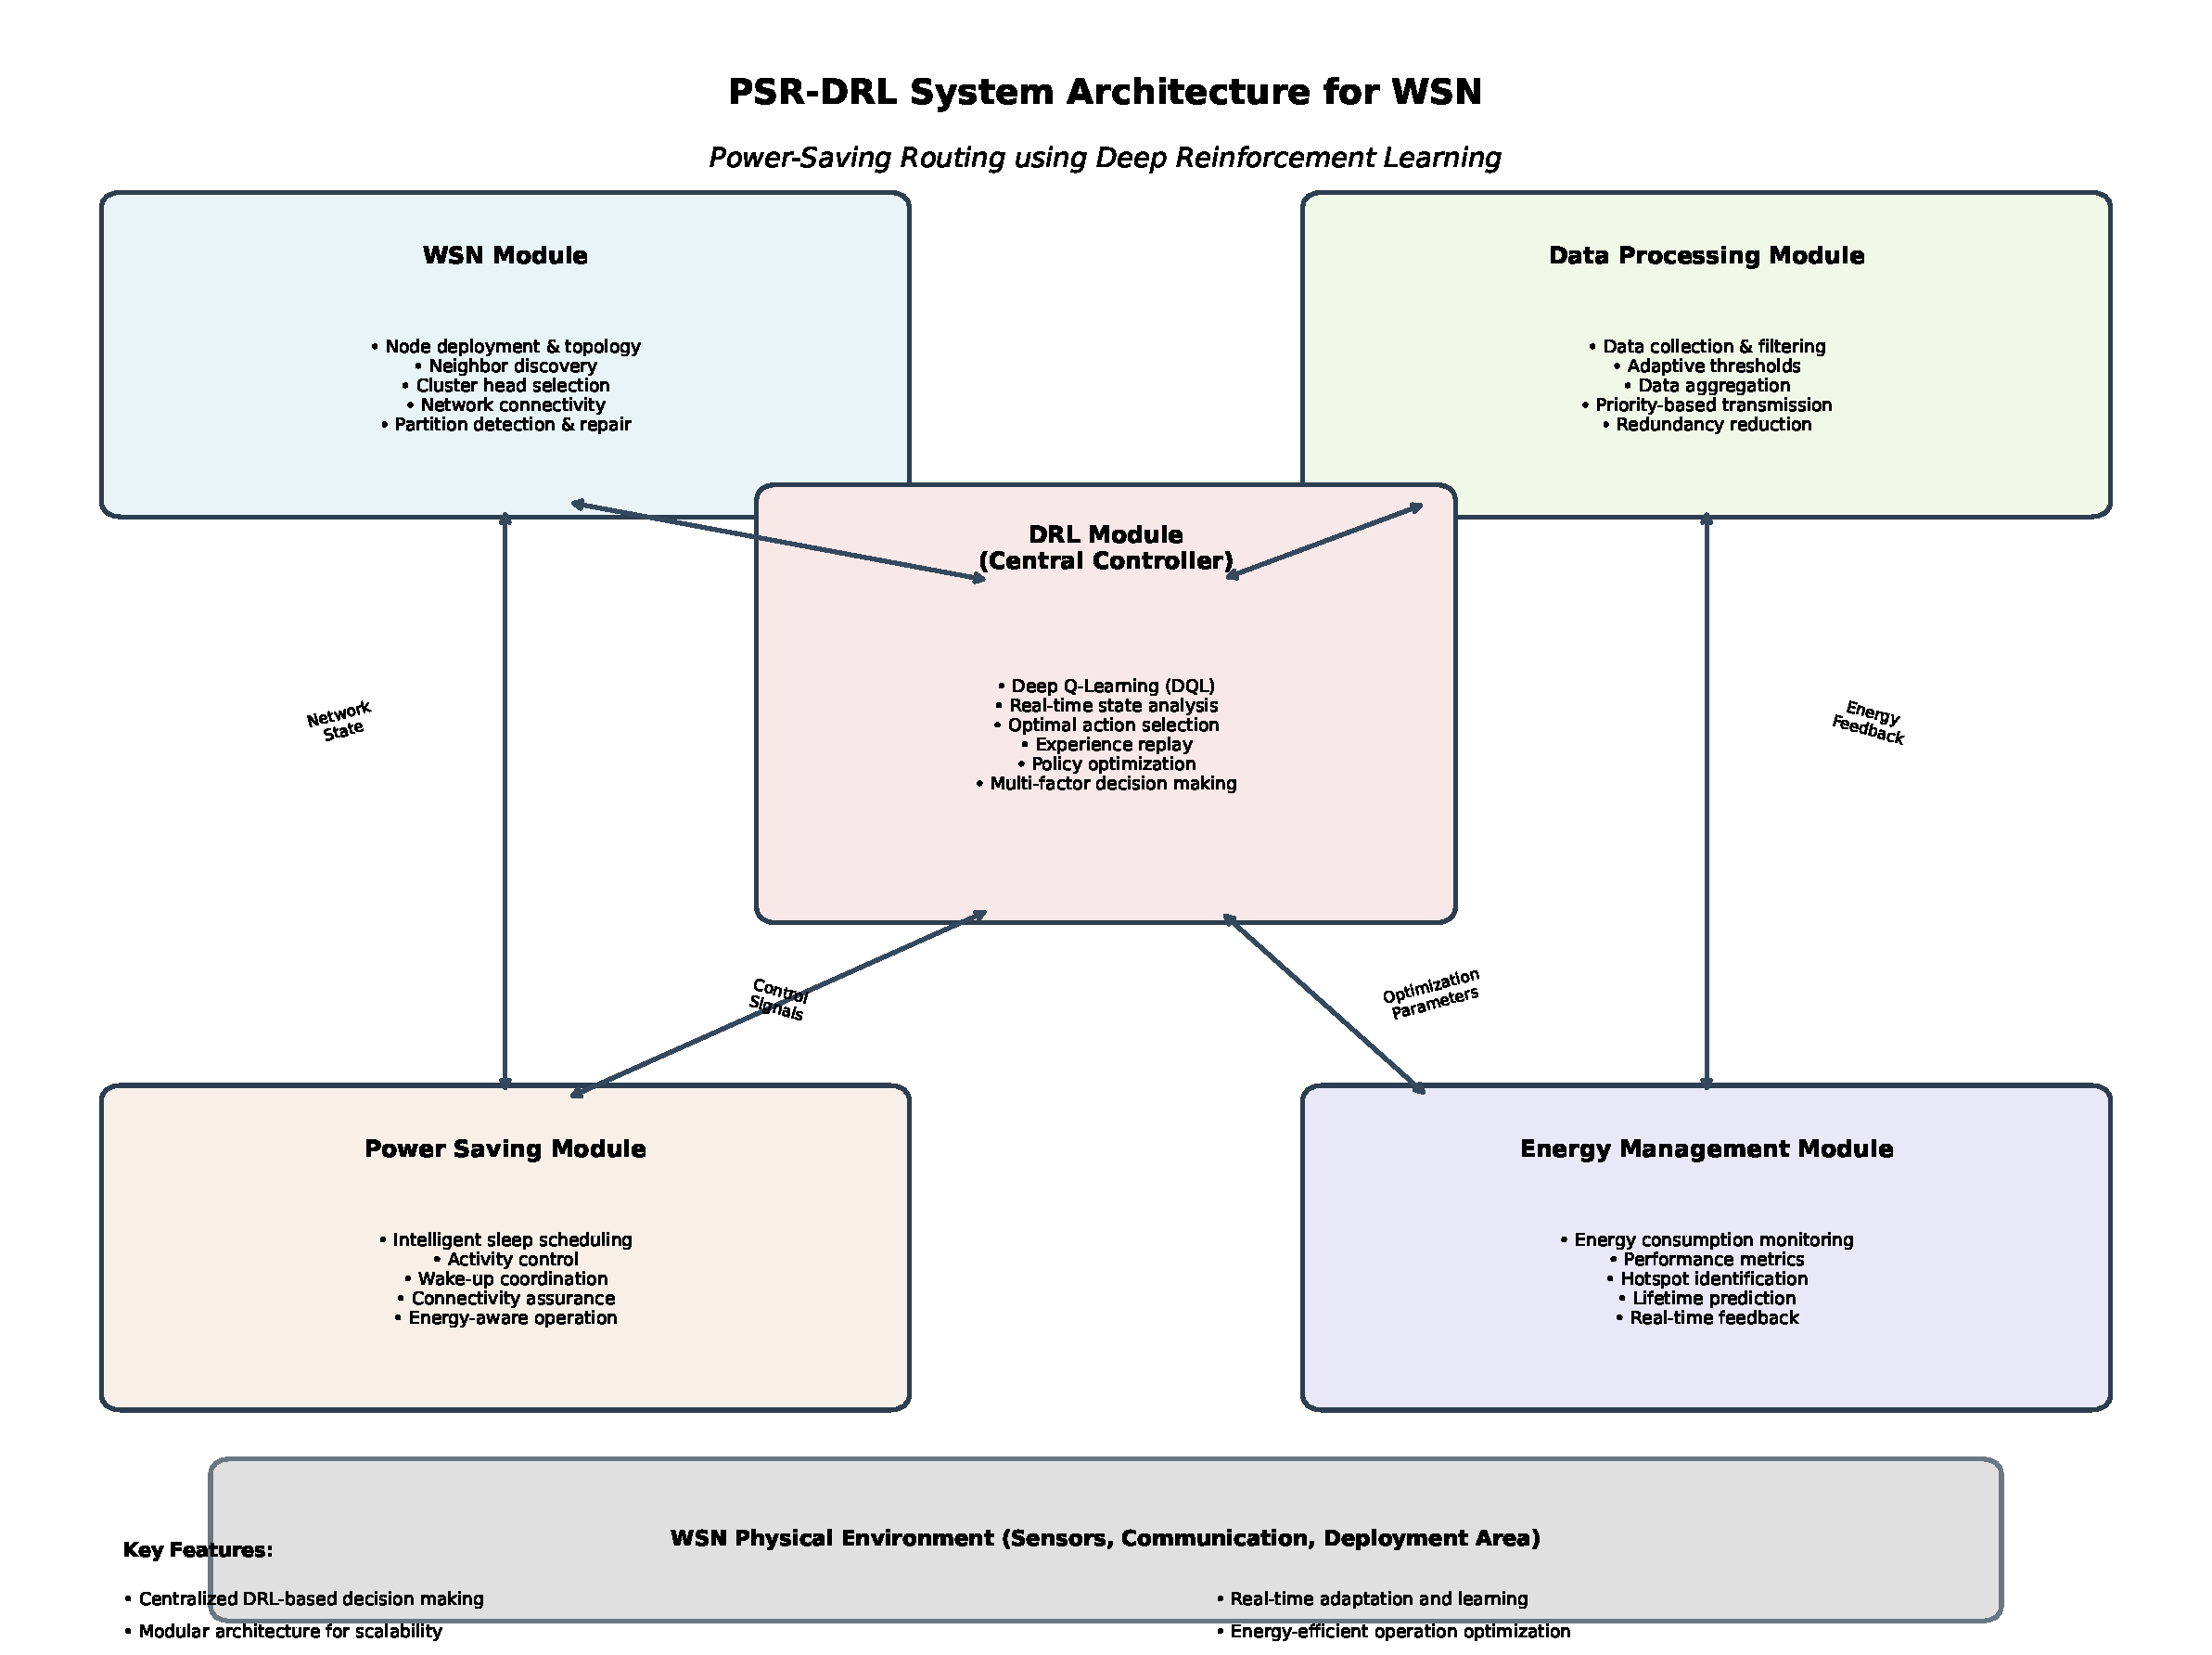
\includegraphics[width=0.95\textwidth]{All figures/PSR_DRL_System_Architecture.pdf}
    \caption{PSR-DRL System Architecture showing the five core modules and their interactions. The DRL module serves as the central controller, receiving inputs from all other modules and providing optimized decisions for routing and power management.}
    \label{fig:psr_drl_architecture}
\end{figure}

\subsection{Core System Modules}

\textbf{WSN Module:}  
This module sets up and controls the sensor network's physical and logical layout. It takes care of deploying nodes, finding neighbors, and keeping the network connected. It chooses cluster heads \cite{abadi2022rlbeep, mutombo2021eer, 10717297} depending on the energy of the nodes and their position in the network. It also changes the membership of the clusters and rotates leadership to ensure that energy use is balanced \cite{8474286}. The module also finds and fixes network partitions, which keeps the system strong even when nodes fail or move \cite{YICK20082292}.

The WSN module implements distributed algorithms for:
\begin{itemize}
    \item Network topology discovery and maintenance
    \item Dynamic cluster formation based on energy and proximity
    \item Neighbor discovery protocols with adaptive intervals
    \item Network partition detection and self-healing mechanisms
    \item Quality of Service (QoS) maintenance across the network
\end{itemize}

\textbf{Data Processing Module:}  
This module is responsible for gathering, sifting, and combining sensor data \cite{8057520}. It decides which data is important enough to send \cite{AHMED2017242}. It employs adaptive thresholds to filter out unimportant information by taking into account changes in sensor readings and the situation \cite{8057520}. At cluster heads, data aggregation reduces redundancy and transmission burden \cite{moon2017}. It also ensures that critical or urgent data is delivered reliably, even when the network is busy \cite{10406923}.

Key functionalities include:
\begin{itemize}
    \item Real-time data filtering using adaptive thresholds
    \item Statistical and semantic data aggregation at cluster heads
    \item Priority-based data classification for transmission scheduling
    \item Data compression algorithms to reduce communication overhead
    \item Redundancy elimination through spatial and temporal correlation
\end{itemize}

\textbf{DRL Module:} This module uses DQL \cite{vijayanpv2020deep, 8243989} to examine the real-time network's condition and determine the optimal actions for routing and energy management. It is the central part of the system's decision-making process \cite{9014179, MAZYAVKINA2021105400}. It takes into account several things, like residual energy, distance, congestion, and data urgency \cite{doi:10.1177/1550147719833541}. It uses a learned policy that becomes better over time through experience replay and reward feedback \cite{8701570}. The module chooses between routing paths and sleep modes to achieve the best long-term performance of the network and spread the energy use evenly across all nodes \cite{9231883}.

The DRL module architecture consists of:
\begin{itemize}
    \item \textbf{State Space}: Multi-dimensional representation including node energy levels, network topology, data urgency, congestion metrics, and connectivity status
    \item \textbf{Action Space}: Discrete and continuous actions for route selection, power level adjustment, and sleep scheduling
    \item \textbf{Deep Q-Network}: Multi-layer neural network with experience replay buffer for policy learning
    \item \textbf{Reward Function}: Multi-objective optimization considering energy efficiency, data delivery success, and network longevity
    \item \textbf{Exploration Strategy}: Adaptive $\epsilon$-greedy policy with decay for exploration-exploitation balance
\end{itemize}

\textbf{Power Saving Module:}  
This module sets up smart sleep schedules and activity controls for each node. The module determines when nodes should go to sleep or wake up by monitoring their recent activity, energy level, and network requirements. Sleep scheduling \cite{abadi2022rlbeep, SACHITHANANDAM2025101071} is tailored to each user, making sure there are enough active nodes for connectivity while saving the most energy \cite{s24061993}. The module organizes wake-up events to help with timely data delivery and network upkeep \cite{9292984}.

Advanced power management features:
\begin{itemize}
    \item Coordinated sleep scheduling to maintain network connectivity
    \item Dynamic duty cycle adjustment based on network traffic
    \item Energy-aware wake-up protocols for critical events
    \item Predictive sleep planning using historical data patterns
    \item Emergency wake-up mechanisms for network maintenance
\end{itemize}

\textbf{Energy Management Module:}  
This module monitors and enhances the energy consumption of the network \cite{a13030072}. It does this by recording how much energy is used for all network activity, such as sending, receiving, processing, and sleeping \cite{AKKAYA2005325}. It determines comprehensive performance indicators, identifies energy hotspots, and predicts the network's lifespan based on its current usage \cite{7374157}. The module provides the DRL module with real-time feedback, enabling it to adjust its routing and sleep methods to prevent node failures and maintain network operation for as long as possible \cite{9474495}.

Comprehensive energy monitoring includes:
\begin{itemize}
    \item Real-time energy consumption tracking for all network operations
    \item Energy hotspot identification and load balancing recommendations
    \item Network lifetime prediction using statistical and machine learning models
    \item Energy efficiency metrics calculation and reporting
    \item Adaptive energy threshold management for different network conditions
\end{itemize}

\subsection{System Operation Flow}

Figure~\ref{fig:psr_drl_flow} demonstrates the operational flow of the PSR-DRL system, showing how the modules interact in a continuous cycle of data collection, analysis, decision-making, and optimization.

\begin{figure}[htbp]
    \centering
    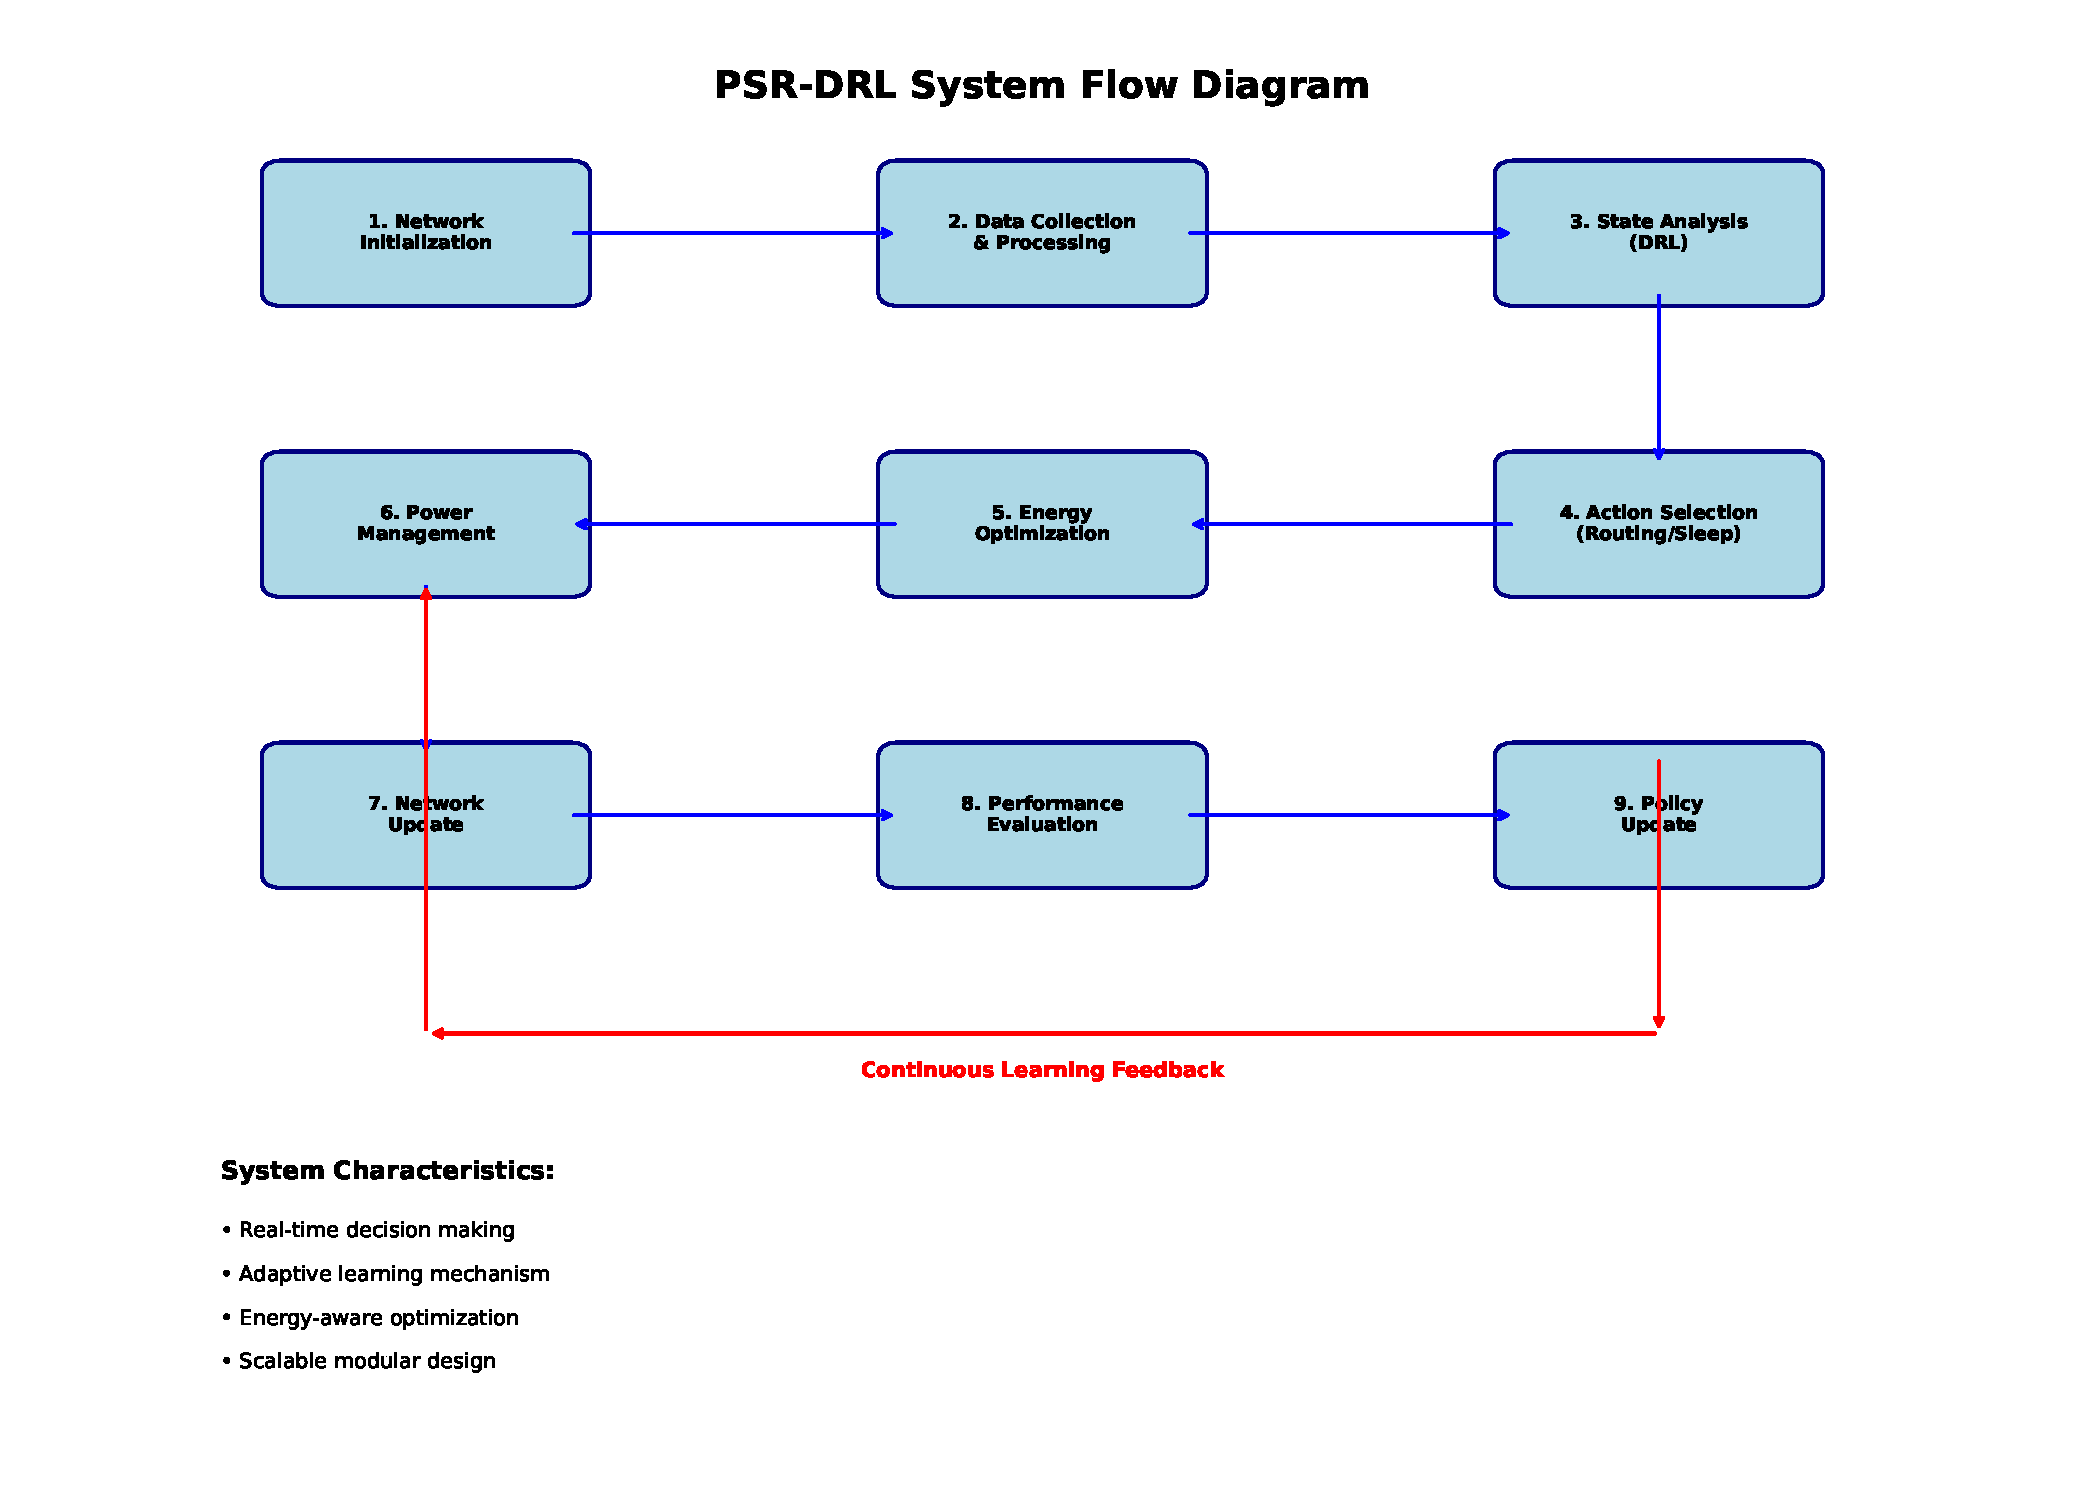
\includegraphics[width=0.9\textwidth]{All figures/PSR_DRL_Flow_Diagram.pdf}
    \caption{PSR-DRL System Operation Flow Diagram illustrating the nine-step process from network initialization to policy updates, with continuous learning feedback for adaptive optimization.}
    \label{fig:psr_drl_flow}
\end{figure}

The system operates through the following phases:

\textbf{Initialization Phase:} Network setup, node deployment, and initial cluster formation based on energy levels and spatial distribution.

\textbf{Data Collection Phase:} Continuous monitoring of network state, including energy levels, topology changes, data traffic, and environmental conditions.

\textbf{Analysis Phase:} The DRL module processes collected information to understand current network state and predict optimal actions.

\textbf{Decision Phase:} Selection of optimal routing paths and power management strategies using the trained deep Q-network.

\textbf{Execution Phase:} Implementation of selected actions through coordinated module operations.

\textbf{Evaluation Phase:} Performance assessment and reward calculation based on multiple objectives.

\textbf{Learning Phase:} Policy updates through experience replay and neural network parameter adjustment.

\textbf{Adaptation Phase:} System-wide parameter adjustments based on learned experiences and changing network conditions.

\subsection{Inter-Module Communication Protocol}

The modules communicate through a well-defined message-passing protocol that ensures efficient information exchange while maintaining system modularity:

\begin{itemize}
    \item \textbf{Synchronous Communication}: Critical real-time decisions requiring immediate response
    \item \textbf{Asynchronous Communication}: Non-critical updates and background monitoring
    \item \textbf{Event-Driven Communication}: Emergency situations and threshold-based alerts
    \item \textbf{Periodic Communication}: Regular status updates and performance reports
\end{itemize}

\subsection{System Performance Characteristics}

The PSR-DRL system is designed to meet the following performance requirements:

\begin{itemize}
    \item \textbf{Real-time Response}: Decision-making within 100ms for routing decisions
    \item \textbf{Scalability}: Support for networks ranging from 10 to 1000 nodes
    \item \textbf{Energy Efficiency}: System overhead less than 5\% of total network energy
    \item \textbf{Adaptability}: Automatic adjustment to network topology changes
    \item \textbf{Reliability}: 99.9\% uptime with graceful degradation capabilities
\end{itemize}

\vspace{0.5em}
In conclusion, the PSR-DRL system model brings various specialized modules together into a single, flexible design. Each module is crucial for achieving the right balance between energy efficiency and reliability, ensuring that WSNs can operate effectively, grow, and remain robust in dynamic real-world environments. The modular architecture enables independent optimization of each component while maintaining system-wide coherence through the central DRL-based decision-making framework.
